\section{Results}
\subsection{Cornell Box Experiment Results}
The resulting generated images show promising results for deep learning aided in situ scientific visualisation. We observe the network successfully learned to emulate light transport in a realistic fashion with offline performance as can be seen in the highlighted region of figure \ref{fig:lighttransport}.

\begin{figure}
    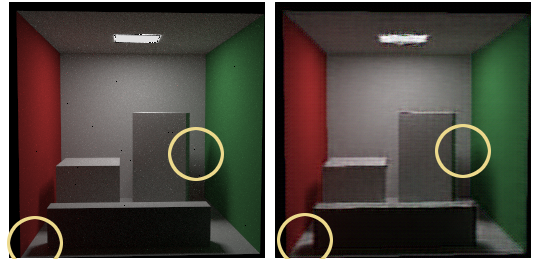
\includegraphics[width=0.55\textwidth]{genDemo.png}
    \caption{Ground truth path traced image \textbf{(left)} and image generated from noise and conditional buffers by cGAN \textbf{(right)}.}
    \label{fig:lighttransport}
\end{figure}

What is more, though designed in a ``one network for one scene'' setting, the generative net proved to be adaptive and able to generate accurate renderings for not only unobserved camera orientation renderings during training but also varied scenes of a similar flavor when provided the conditional geometry buffers of the novel scene. 
%\vspace{-1.5em}
\begin{figure}
\centering
\begin{subfigure}{.5\textwidth}
\centering
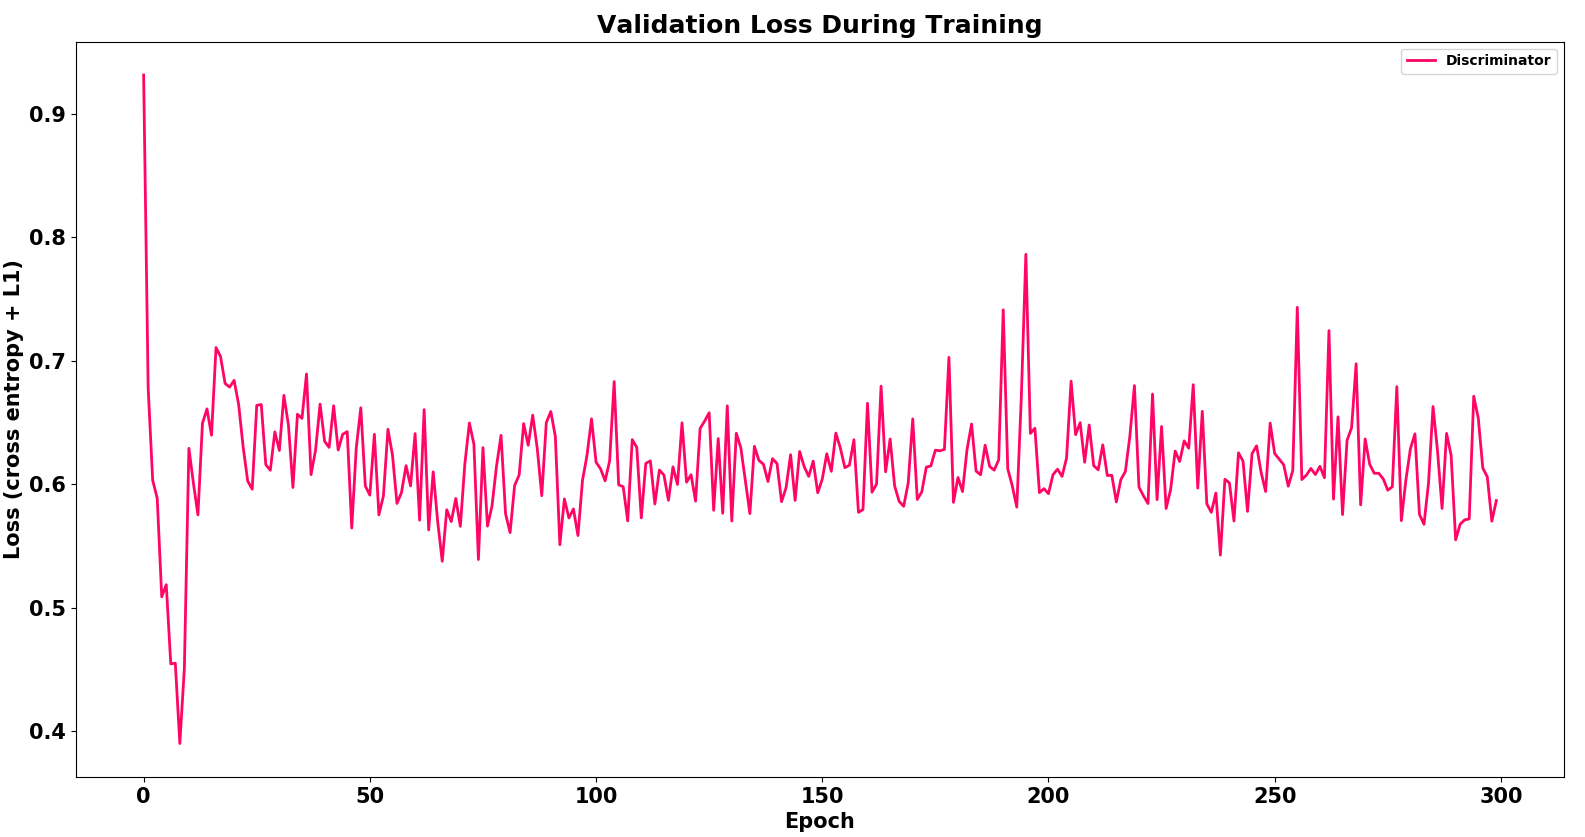
\includegraphics[width=.9\textwidth]{discrimloss.png}
\end{subfigure}
\begin{subfigure}{.5\textwidth}
\centering
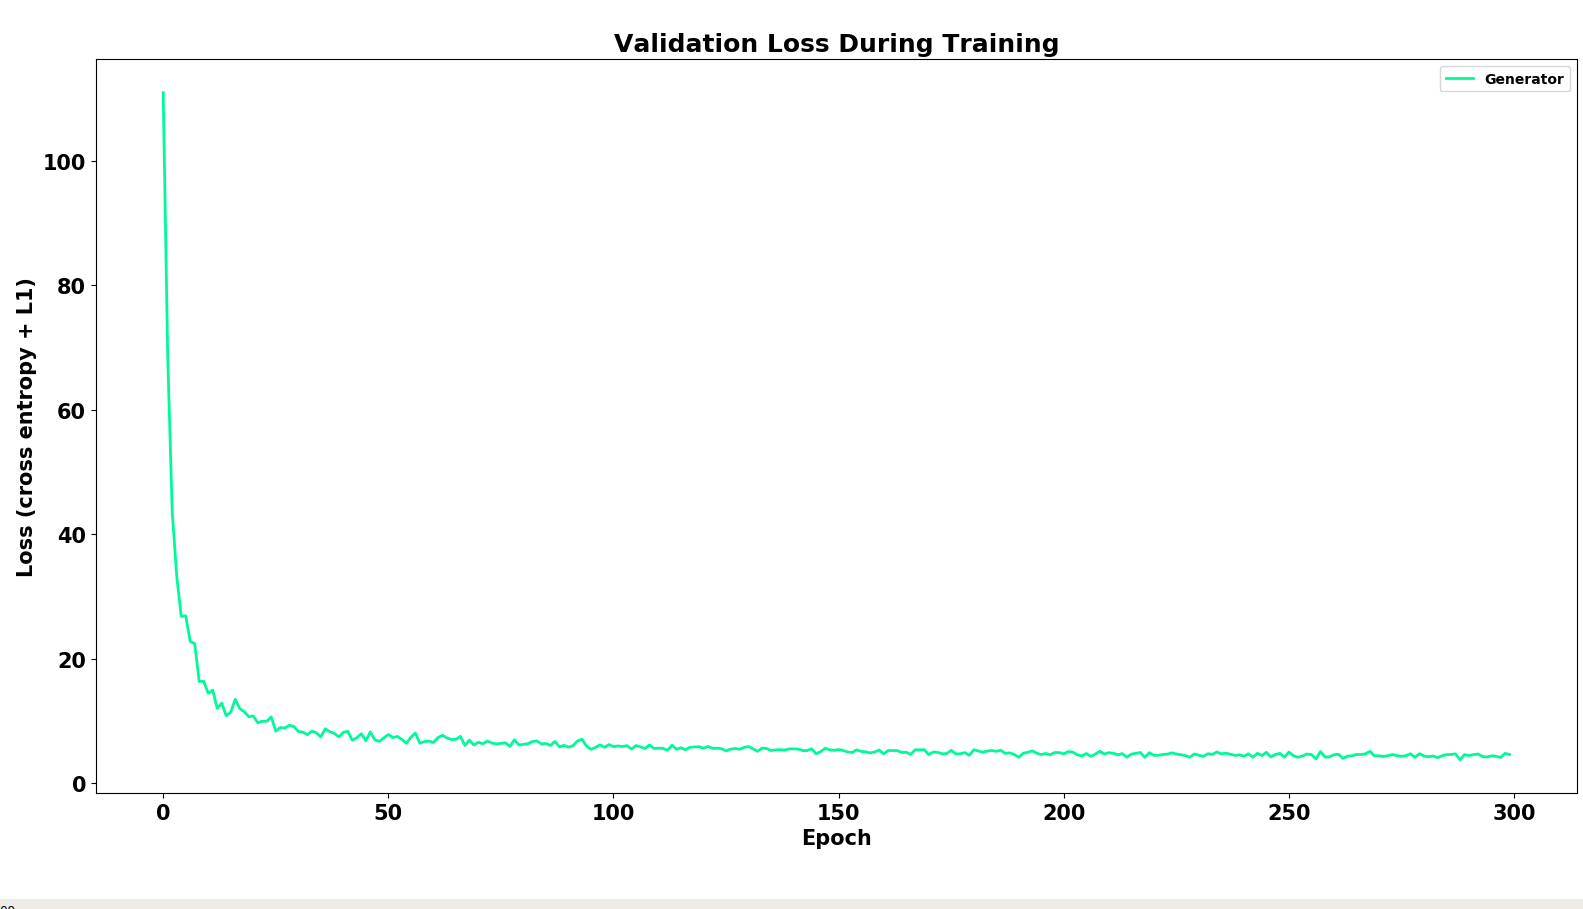
\includegraphics[width=.9\textwidth]{genloss.png}
\end{subfigure}
\caption{Generator loss converging to 0 and discriminator loss converging to 0.5 corresponding to inability to differentiate real from generated images.}
\end{figure}


\subsection{Solution Design Assessment}


3080 256x256 high quality ground truth images were rendered utilizing the VTK-m path tracer and two Nvidia RTX-2080 Ti GPUs requiring 12 hours. To generate 3080 images, a camera was positioned in a hemisphere around the Cornell Box, and moved along the hemisphere as the camera consistent ``looked'' at the center of the Cornell Box. This was the ground truth training set for the cGAN. Each image was considered a single datum in the path traced training set.

%17471.48user 9708.75system 4:26:31elapsed 169%CPU (0avgtext+0avgdata 13497260maxresident)

Training the cGAN on this image data set over 400 epochs using one GPU on the same machine took 9709 seconds. %Once trained the run time of applying the generative U-Net provided the conditional buffer set averages \_\_\_ seconds. 



